% !TeX root = main-limak-thesis.tex

%%%%%%%%%%%%%%%%%%%%%%%%%%%%%%%%%%%%%%%%%%%%%%%%%%%%%%%%%%%%%%%%%%%%%%%%%%%%%%%%
%% KAPITEL 7: EVALUATION UND ERGEBNISSE
%%
%% Gemäß LIMAK Leitfaden: Präsentation und Analyse der Ergebnisse
%%
%% Tipps:
%% - Strukturierte Darstellung der erhobenen Daten
%% - Quantitative Ergebnisse mit Tabellen und Grafiken visualisieren
%% - Qualitative Ergebnisse systematisch aufbereiten
%% - Vergleich mit definierten Zielen/Hypothesen
%% - Objektive Darstellung ohne Interpretation (kommt in Diskussion)
%%%%%%%%%%%%%%%%%%%%%%%%%%%%%%%%%%%%%%%%%%%%%%%%%%%%%%%%%%%%%%%%%%%%%%%%%%%%%%%%

\chapter{Evaluation und Ergebnisse}
\label{chap:evaluation}

%% TODO: Passen Sie die Abschnitte an Ihre Forschungsmethodik an und ersetzen Sie
%% alle Platzhalter [...] mit Ihren eigenen Daten und Ergebnissen.

%% Kurze Einleitung zum Kapitel
Dieses Kapitel präsentiert die Ergebnisse der empirischen Untersuchung. Zunächst wird in Abschnitt~\ref{sec:eval-methodik} die Evaluationsmethodik beschrieben. Abschnitt~\ref{sec:quantitative-ergebnisse} stellt die quantitativen Ergebnisse dar, während Abschnitt~\ref{sec:qualitative-ergebnisse} die qualitativen Befunde zusammenfasst. Abschließend erfolgt in Abschnitt~\ref{sec:zielerreichung} eine Bewertung der Zielerreichung.

\section{Evaluationsmethodik}
\label{sec:eval-methodik}

Die Evaluation erfolgte im Zeitraum [Monat/Jahr] bis [Monat/Jahr] anhand der in Kapitel~\ref{chap:methodik} definierten Kennzahlen und Kriterien.

%% Beschreiben Sie hier:
%% - Evaluationszeitraum
%% - Verwendete Instrumente (Fragebögen, Interviews, Messungen)
%% - Stichprobengröße und -zusammensetzung
%% - Durchführung der Datenerhebung

\section{Quantitative Ergebnisse}
\label{sec:quantitative-ergebnisse}

\subsection{[Ergebnisbereich 1]}

%% Beispiel: Durchlaufzeiten, Kosten, Kennzahlen, Umfrageergebnisse

\begin{table}[htbp]
\centering
\begin{tabular}{@{}lccc@{}}
\toprule
\textbf{Kennzahl} & \textbf{Vorher} & \textbf{Nachher} & \textbf{Veränderung} \\
\midrule
{[Kennzahl 1]} & {[X]} & {[Y]} & {[+/-Z]\%} \\
{[Kennzahl 2]} & {[X]} & {[Y]} & {[+/-Z]\%} \\
{[Kennzahl 3]} & {[X]} & {[Y]} & {[+/-Z]\%} \\
{[Kennzahl 4]} & {[X]} & {[Y]} & {[+/-Z]\%} \\
\bottomrule
\end{tabular}
\caption{Vorher-Nachher-Vergleich [Beschreibung]}
\label{tab:vergleich-ergebnisse}
\end{table}

\textbf{Beschreibung der Ergebnisse:}
[Kurze sachliche Beschreibung der in der Tabelle dargestellten Ergebnisse ohne Interpretation]

%% Beispiel für ein Balkendiagramm mit TikZ
Abbildung~\ref{fig:beispiel-diagramm} visualisiert die Entwicklung über drei Perioden:

\begin{figure}[htbp]
\centering
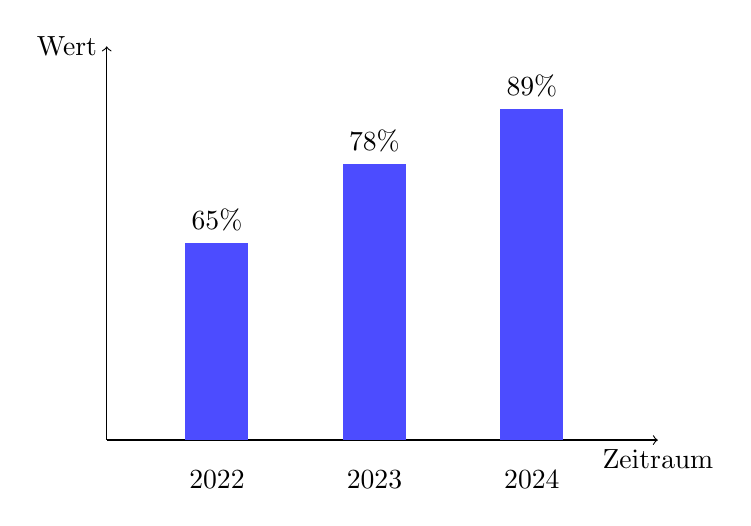
\begin{tikzpicture}
  % Achsen
  \draw[->] (0,0) -- (0,5) node[left] {Wert};
  \draw[->] (0,0) -- (7,0) node[below] {Zeitraum};

  % Balken in LIMAK-Blau
  \fill[blue!70] (1,0) rectangle (1.8,2.5);
  \fill[blue!70] (3,0) rectangle (3.8,3.5);
  \fill[blue!70] (5,0) rectangle (5.8,4.2);

  % Beschriftungen
  \node at (1.4,-0.5) {2022};
  \node at (3.4,-0.5) {2023};
  \node at (5.4,-0.5) {2024};

  % Werte
  \node at (1.4,2.8) {65\%};
  \node at (3.4,3.8) {78\%};
  \node at (5.4,4.5) {89\%};
\end{tikzpicture}
\caption{Beispiel: Entwicklung der Zielerreichung (in \%, eigene Darstellung)}
\label{fig:beispiel-diagramm}
\end{figure}

\subsection{[Ergebnisbereich 2]}

\begin{table}[htbp]
\centering
\begin{tabular}{@{}lcc@{}}
\toprule
\textbf{Kriterium} & \textbf{Messwert} & \textbf{Zielwert} \\
\midrule
{[Kriterium 1]} & {[X]} & {[Y]} \\
{[Kriterium 2]} & {[X]} & {[Y]} \\
{[Kriterium 3]} & {[X]} & {[Y]} \\
\bottomrule
\end{tabular}
\caption{[Beschreibung der Tabelle]}
\label{tab:ergebnisse-2}
\end{table}

\subsection{Statistische Auswertung}

%% Falls statistische Tests durchgeführt wurden:
%% - Deskriptive Statistik (Mittelwerte, Standardabweichungen)
%% - Inferenzstatistik (t-Tests, ANOVA, Korrelationen)
%% - Signifikanzniveaus

[Beschreibung der statistischen Auswertung und Signifikanztests]

\section{Qualitative Ergebnisse}
\label{sec:qualitative-ergebnisse}

\subsection{Ergebnisse aus Interviews/Befragungen}

%% Beispiel für qualitative Ergebnisse aus Interviews oder offenen Fragen

Die Auswertung der [X] durchgeführten Interviews ergab folgende Hauptkategorien:

\begin{description}
    \item[Kategorie 1:] [Beschreibung der Erkenntnisse]
    \item[Kategorie 2:] [Beschreibung der Erkenntnisse]
    \item[Kategorie 3:] [Beschreibung der Erkenntnisse]
\end{description}

%% Beispielzitate aus Interviews (anonymisiert):
\begin{quote}
``[Anonymisiertes Zitat eines Interviewpartners]'' (Interview [X])
\end{quote}

\subsection{Beobachtungen}

%% Falls Beobachtungen durchgeführt wurden:
[Zusammenfassung der dokumentierten Beobachtungen]

\section{Kostenbewertung}
\label{sec:kosten}

%% Falls eine Kosten-Nutzen-Analyse Teil der Arbeit ist:

\subsection{Implementierungskosten}

\begin{table}[htbp]
\centering
\begin{tabular}{@{}lc@{}}
\toprule
\textbf{Kostenposition} & \textbf{Betrag (EUR)} \\
\midrule
{[Position 1]} & {[X]} \\
{[Position 2]} & {[X]} \\
{[Position 3]} & {[X]} \\
\midrule
\textbf{Gesamt} & \textbf{[X]} \\
\bottomrule
\end{tabular}
\caption{[Beschreibung der Kostentabelle]}
\label{tab:kosten}
\end{table}

\subsection{Return on Investment}

%% Falls relevant:
[Berechnung und Darstellung des ROI]

\section{Zielerreichung}
\label{sec:zielerreichung}

%% Systematischer Abgleich der Ergebnisse mit den in Kapitel 1 definierten Zielen

\begin{table}[htbp]
\centering
\begin{tabular}{@{}lcc@{}}
\toprule
\textbf{Ziel} & \textbf{Zielvorgabe} & \textbf{Erreicht} \\
\midrule
{[Ziel 1]} & {[Vorgabe]} & {[Ja/Teilweise/Nein]} \\
{[Ziel 2]} & {[Vorgabe]} & {[Ja/Teilweise/Nein]} \\
{[Ziel 3]} & {[Vorgabe]} & {[Ja/Teilweise/Nein]} \\
{[Ziel 4]} & {[Vorgabe]} & {[Ja/Teilweise/Nein]} \\
\bottomrule
\end{tabular}
\caption{Übersicht der Zielerreichung}
\label{tab:zielerreichung}
\end{table}

\section{Lessons Learned}
\label{sec:lessons-learned}

\subsection{Erfolgsfaktoren}
\begin{itemize}
    \item {[Erfolgsfaktor 1]}
    \item {[Erfolgsfaktor 2]}
    \item {[Erfolgsfaktor 3]}
\end{itemize}

\subsection{Herausforderungen}
\begin{itemize}
    \item {[Herausforderung 1]}
    \item {[Herausforderung 2]}
    \item {[Herausforderung 3]}
\end{itemize}

\subsection{Optimierungspotenziale}
\begin{itemize}
    \item {[Potenzial 1]}
    \item {[Potenzial 2]}
    \item {[Potenzial 3]}
\end{itemize}

